\documentclass[11pt,a4paper]{article}
\usepackage[utf8x]{inputenc}
\usepackage{amsmath}
\usepackage{amsfonts}
\usepackage{graphicx}
\usepackage[table,xcdraw]{xcolor}


\usepackage{caption}
\usepackage{subcaption}

\renewcommand{\familydefault}{\sfdefault} % cambiamos la fuente a una sans

\usepackage{float} % para que floten las imagenes o algo asi...
\usepackage{wallpaper} %paquete para usar una imagen como encabezado!
\usepackage{hyperref} %para usar hypervinculos 
\usepackage[export]{adjustbox} %para usar marcos en imagenes
\usepackage{eurosym} % para el euro
\usepackage{transparent} %para las marcas de agua
\usepackage{eso-pic}  %para las marcas de agua

\definecolor{azul_marcos}{RGB}{0,128,159} %defino el color azul de los marcos
\usepackage{sectsty} %esto es para cambiar el color de las fuentes creo
\renewcommand{\familydefault}{\sfdefault} % cambiamos la fuente a una sans
\sectionfont{\color{azul_marcos}}  % sets colour of sections
\subsectionfont{\color{azul_marcos}}  % sets colour of sections


\usepackage{pdfpages} %para insertar pdfs
\usepackage{amssymb}
\usepackage{pstcol} % para color
\usepackage{pst-node} % para diagramas
\usepackage{pst-plot} % para representacion de dat
\usepackage[spanish]{babel}
\addto\captionsspanish{\renewcommand\chaptername{Bloque}}
%\usepackage[total={18cm,21cm},top=2cm, left=2cm]{geometry}
\usepackage{anysize}
\pagestyle{plain}
%\markboth{left head}{right head}
%\markright{Guía de impresión FlexiSMART}
\marginsize{3cm}{2cm}{2.5cm}{1cm}
\title{Guía do impressão FlexiSMART}
\date{}

%configuracion de la marca de agua
\AddToShipoutPicture{
    \put(0,0){
        \parbox[b][\paperheight]{\paperwidth}{%
            \vfill
            \centering
            {\transparent{0.2}
\includegraphics[scale=1.25]{FOTOS/logofff}}%
            \vfill
        }
    }
}

\begin{document}
\ULCornerWallPaper{1}{FOTOS/header}
\LLCornerWallPaper{1}{FOTOS/footer}
%\maketitle
%\tableofcontents

\includepdf{PDF/EN_PORTADA.pdf}
\section{O que é o FlexiSMART?}FlexiSMART é um filamento para impressão 3D FFF/FDM fabricado a partir de polímeros elastómeros termoplásticos (TPE) com aditivos químicos para facilitar a impressão na maioria das impressoras 3D do mercado.
\\\\
FlexiSMART é flexível e recupera a sua forma ao dobrá-lo, retorcê-lo ou esticá-lo.

\section{Porquê usar FlexiSMART?}
FlexiSMART permite-lhe entrar num novo mundo de possibilidades, graças à natureza flexível do filamento. A partir de agora pode imprimir objetos que antes, com um filamento rígido, não podia: capas de smartphones, tablets, sapatilhas, palmilhas, rodas para carros telecomandados, próteses, silent blocks, engrenagens que necessitem de uma certa adaptabilidade e, em geral, qualquer objeto que lhe ocorra e que possa fazer uso das suas propriedades.
\\\\
FlexiSMART foi concebido para ser fácil de imprimir:
\begin{itemize}
\item Tem uma certa rigidez, para que possa ser impresso pela maioria dos extrusores diretos, com poucas ou nenhumas modificações.
\item A aderência é excelente. Pode imprimir inclusivamente sem cama quente.
\item A resistência é muito alta, pelo que as peças impressas não se degradarão rapidamente.
\item É o filamento flexível com os preços mais atrativos da Europa.
\end{itemize}

\section{Ficha técnica e parâmetros de impressão}

\begin{table}[H]
\centering
\caption*{Ficha técnica}
\begin{tabular}{|
>{\columncolor[HTML]{FFFFFF}}l |
>{\columncolor[HTML]{FFFFFF}}c |}
\hline
\multicolumn{1}{|c|}{\cellcolor[HTML]{FFFFFF}\textbf{Material}}   & FlexiSMART (TPE)   \\ \hline
\textbf{Cores disponiveis}              & 11                 \\ \hline
\textbf{Formatos disponíveis}             & 1kg, 250gr         \\ \hline
\textbf{Temperatura de deflexão térmica} & 90ºC               \\ \hline
\textbf{Temperatura de fusão}            & 160ºC              \\ \hline
\textbf{Temperatura de decomposição}    & \textgreater 240ºC \\ \hline
\textbf{Densidade}                         & 0.96 gr / cm3      \\ \hline
\textbf{Alongamento máximo}              & 600\%              \\ \hline
\end{tabular}
\end{table}
\begin{table}[H]
\centering
\caption*{Parâmetros de impressão recomendados usando um nozzle de 0.4 mm}
\begin{tabular}{|
>{\columncolor[HTML]{FFFFFF}}l |
>{\columncolor[HTML]{FFFFFF}}c |}
\hline
\multicolumn{1}{|c|}{\cellcolor[HTML]{FFFFFF}\textbf{Temperatura de impressão recomendada}} & 195º-220º              \\ \hline
\textbf{Velocidade de impressão recomendada}                         & 20-60mm/s              \\ \hline
\textbf{Temperatura do leito quentes}                                  & \textgreater 18º        \\ \hline
\textbf{Camada óptima altura}                                      & 0.2 mm                 \\ \hline
\textbf{Perímetros}                                                 & 3                      \\ \hline
\textbf{Top solid layers}                                           & 5                      \\ \hline
\textbf{Retração}                                                 & Desativado ou reduzido \\ \hline
\end{tabular}
\end{table}

Pode descarregar os nossos perfis completos de impressão dos principais programas de laminação (Cura, Slic3r e Simplify3D) no nosso site:
\\\\
\centerline{ {\huge \url{www.fffworld.com/documentation} } }
\\\\
Os parâmetros ótimos dependerão da impressora 3D que você utilize, no entanto, são uns bons parâmetros para tomar como ponto de partida. Com umas poucas impressões será capaz de encontrar os limites e a configuração perfeita para a sua máquina.
\section{Problemas e Soluções}
	\subsection{Problemas ao extrudir FlexiSMART}
O principal desafio na hora de imprimir FlexiSMART e outros filamentos flexíveis deriva da própria natureza do material, já que, ao ser flexível, não pode ser empurrado com a mesma facilidade que os materiais rígidos, da mesma forma que não se consegue empurrar uma corda.
\\\\
O problema dá-se quando há folgas em certas partes do extrusor, em particular, entre a drive-gear (a roda dentada que empurra o filamento) e o orifício através do qual o filamento acede ao hot-end (ponta metálica que funde o filamento).
\\\\
Quando este espaço é suficientemente grande, o filamento tende a sair do seu percurso e a formar um nó que acaba por aparecer numa lateral do extrusor, como se pode ver na imagem.
\begin{figure}[H]
\centering
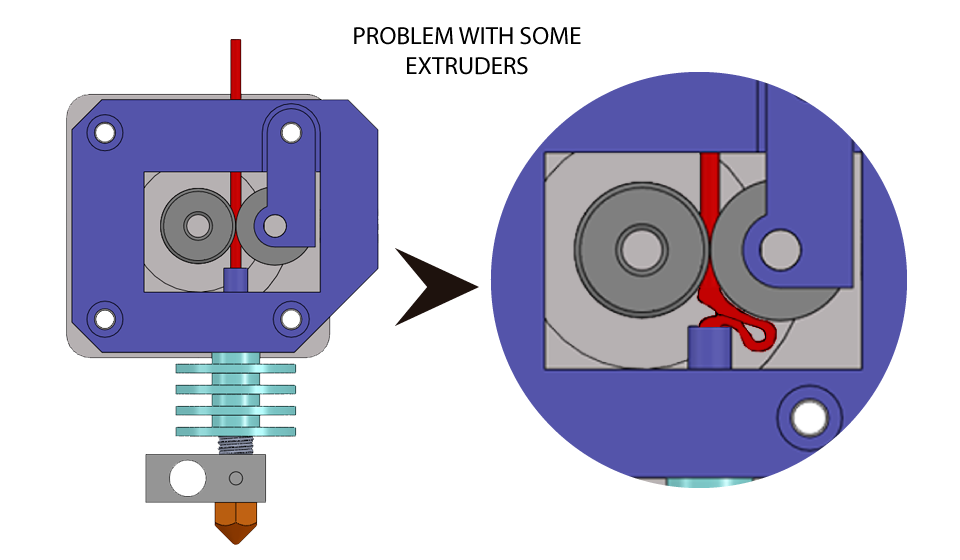
\includegraphics[width=0.5\textwidth,cfbox=azul_marcos 4pt 0pt]{FOTOS/NUDOS1}
\caption*{Extrusor NÃO otimizado para filamentos flexíveis}
\end{figure}
Este problema é maior ao usar filamento de 1.75 mm, já que ao ter menos secção é ainda mais propenso a sair do seu percurso.
\\\\
A velocidade de extrusão é determinante no surgimento deste problema. Se o extrusor empurrar o filamento com demasiada velocidade, cria-se uma pressão para cima que faz com que o filamento saia do seu caminho natural. Por isso a recomendação geral é começar por imprimir a uma velocidade baixa ou muito baixa e ir incrementando-a até encontrar a máxima velocidade que o seu extrusor suporta. O tamanho do nozzle também afeta a velocidade máxima suportada, já que quanto maior for esta, mais material fundido poderá ser extrudido por unidade de tempo e, portanto, maior será a velocidade à qual se pode fazer.
\\\\
Os extrusores concebidos para utilizar filamentos flexíveis minimizam as folgas, impedindo que o filamento possa sair e incorporam um sistema de duplo drive-gear para canalizar com precisão o filamento e evitar completamente o problema mencionado, ao mesmo tempo que permitem aumentar a velocidade de impressão.
\begin{figure}[H]
\centering
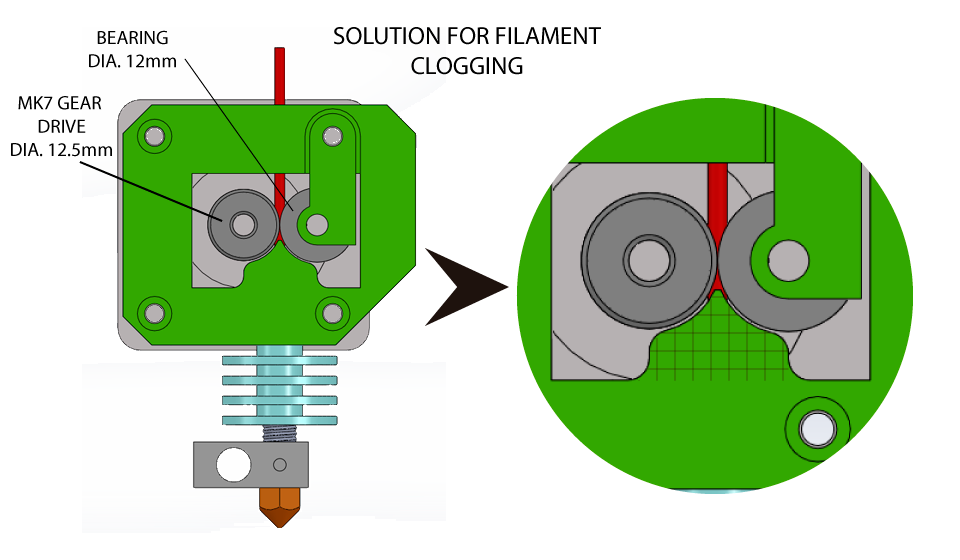
\includegraphics[width=0.5\textwidth,cfbox=azul_marcos 4pt 0pt]{FOTOS/NUDOS2}
\caption*{Extrusor otimizado para filamentos flexíveis}
\end{figure}
\emph{FlexiSMART foi concebido a pensar nestes problemas e tem uma rigidez superior a outros filamentos flexíveis para ajudar a reduzi-los.}
\\\\
No entanto, em extrusores que não estão projetados para usar materiais elásticos, estes problemas podem surgir.
	\subsection{Preparando o extrusor para imprimir FlexiSMART}Se está a ter algum dos problemas anteriormente mencionados, provavelmente tem que adaptar ou substituir o seu extrusor. Neste sentido, existem várias opções que detalhamos a seguir.
		\subsubsection{Modificar o seu extrusor}
Por vezes é possível utilizar FlexiSMART em extrusores não otimizados realizando algumas modificações no mesmo extrusor.
\\\\
Se está a ter problemas para imprimir FlexiSMART sugerimos-lhe que siga os seguintes conselhos, expostos por ordem de complexidade.
			\paragraph{Limar o tubo pelo qual o filamento acede ao hot-end}\mbox{}\\\\
Se usa um extrusor com o corpo de plástico, como os extrusores imprimíveis, recomendamos-lhe que experimente o seguinte. 
\\\\
Lime ligeiramente os bordos do orifício que se encontra mesmo por baixo da drive-gear, orifício através do qual se canaliza o filamento até ao hot-end. Isto permite evitar fricções e enganchamentos que podem provocar os nós anteriormente descritos. 
\\\\
Pode ser necessário desmontar parte do extrusor para realizar esta operação.
			\paragraph{Inserir tubo de teflon no extrusor}\mbox{}\\\\
Uma segunda opção, mais complicada mas mais eficaz, é inserir um tubo de teflon (PTFE) no mencionado orifício. Além disso, esta técnica permite reduzir o espaço com a drive-gear, já que o referido tubo pode colocar-se muito próximo daquela. Inclusivamente pode-se modificar a entrada do tubo de teflon para adaptá-lo à forma do drive-gear, deixando um espaço mínimo.
\\\\
Em geral esta técnica implica furar o extrusor para permitir a inserção do mencionado tubo de teflon. A seguir pode ver imagens do resultado:
\begin{figure}[H]
    \centering
    \begin{subfigure}[b]{0.3\textwidth}
        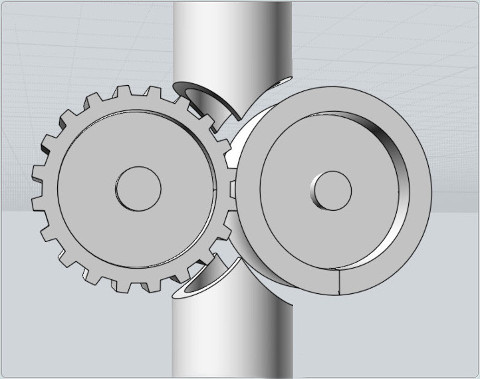
\includegraphics[width=\textwidth,cfbox=azul_marcos 4pt 0pt]{FOTOS/TEFLON1}
    \end{subfigure}
    ~ %add desired spacing between images, e. g. ~, \quad, \qquad, \hfill etc. 
      %(or a blank line to force the subfigure onto a new line)
    \begin{subfigure}[b]{0.3\textwidth}
        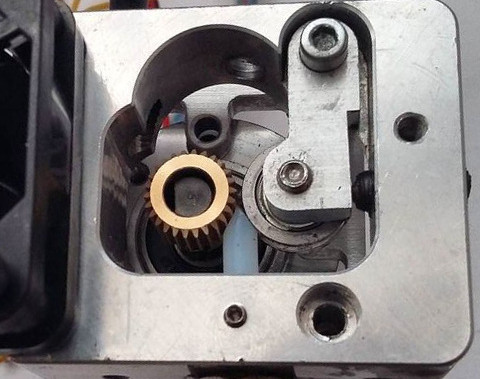
\includegraphics[width=\textwidth,cfbox=azul_marcos 4pt 0pt]{FOTOS/TEFLON2}
    \end{subfigure}
    ~ %add desired spacing between images, e. g. ~, \quad, \qquad, \hfill etc. 
    %(or a blank line to force the subfigure onto a new line)
    \begin{subfigure}[b]{0.3\textwidth}
        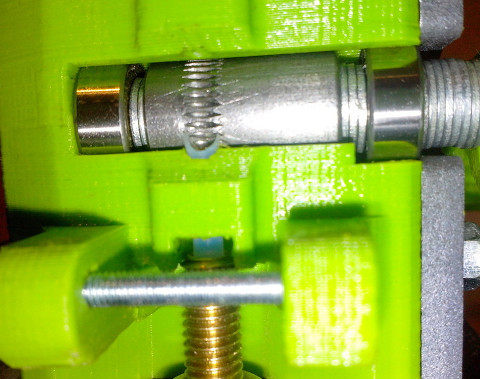
\includegraphics[width=\textwidth,cfbox=azul_marcos 4pt 0pt]{FOTOS/TEFLON3}
    \end{subfigure}
    \caption*{Enxertos de teflon}
\end{figure}
			\paragraph{Imprimir uma guia para o filamento e colocá-la no extrusor}\mbox{}\\\\
A terceira opção é imprimir uma peça que faça de guia para o filamento e colocá-la debaixo do drive-gear. Estas peças têm habitualmente uma forma triangular e devem estar desenhadas respeitando as dimensões de cada extrusor.
\\\\
Na internet, em sites como \url{www.thingiverse.com}, podem descarregar-se este tipo de adaptadores para alguns dos extrusores mais habituais. No entanto, trata-se de um desenho simples que poderá ser criado com facilidade desde o zero por aqueles que tenham conhecimentos de desenho 3D.
\begin{figure}[H]
    \centering
    \begin{subfigure}[b]{0.5\textwidth}
        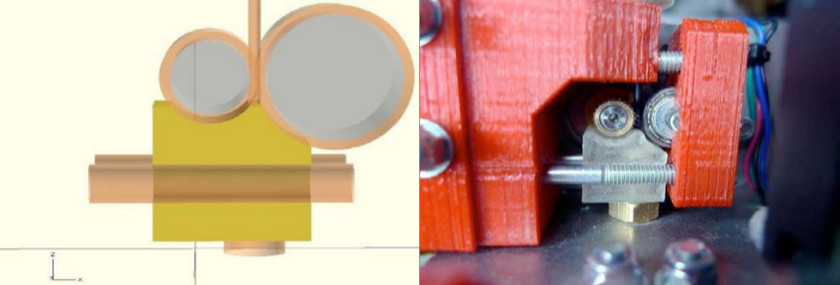
\includegraphics[width=\textwidth,cfbox=azul_marcos 4pt 0pt]{FOTOS/GUIA1}
    \end{subfigure}
    ~ %add desired spacing between images, e. g. ~, \quad, \qquad, \hfill etc. 
      %(or a blank line to force the subfigure onto a new line)
    \begin{subfigure}[b]{0.5\textwidth}
        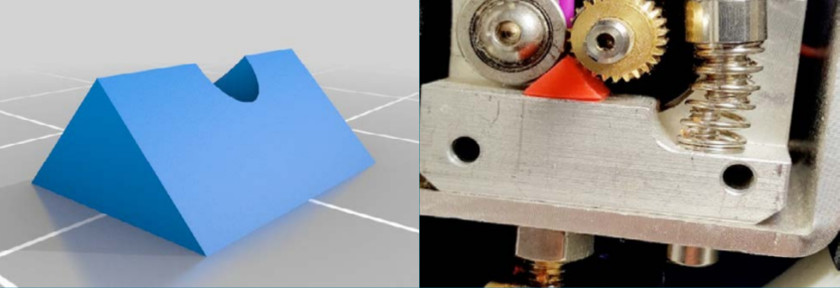
\includegraphics[width=\textwidth,cfbox=azul_marcos 4pt 0pt]{FOTOS/GUIA2}
    \end{subfigure}
    ~ %add desired spacing between images, e. g. ~, \quad, \qquad, \hfill etc. 
    %(or a blank line to force the subfigure onto a new line)
    \begin{subfigure}[b]{0.5\textwidth}
        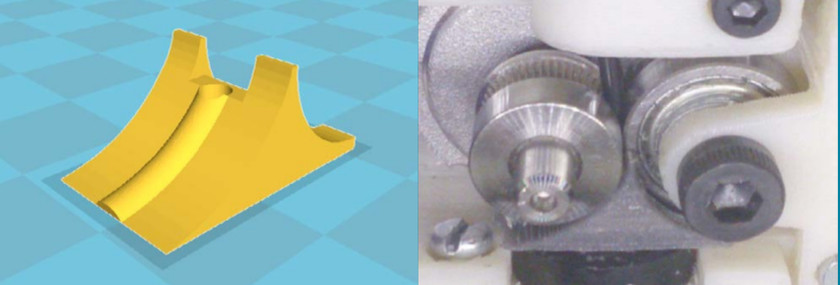
\includegraphics[width=\textwidth,cfbox=azul_marcos 4pt 0pt]{FOTOS/GUIA3}
    \end{subfigure}
    \caption*{Guias de filamento imprimíveis}
\end{figure}	

	\paragraph{Ajustando a pressão do drive-gear sobre o filamento}\mbox{}\\\\
Ao tratar-se de um material flexível é especialmente importante que a pressão do mecanismo que empurra o filamento até ao hot-end não seja excessiva. Nos filamentos rígidos, um excesso de pressão produzirá pequenos entalhes na sua superfície, mas no caso do FlexiSMART uma pressão excessiva deforma a secção do filamento, dando-lhe uma forma ovalada que faz com que se torne propenso a encravar o extrusor.
\\\\
Os extrusores concebidos para a impressão de filamentos flexíveis têm isto em conta e dispõem de um mecanismo para regular a pressão do mecanismo trator. Se o seu extrusor permite regular aquela pressão, recomendamos-lhe que a ajuste ao utilizar FlexiSMART. A pressão adequada será a mínima necessária que permita que o extrusor mova o filamento.
\\\\
Se o seu extrusor não dispõe de mecanismo para regular a pressão, ainda pode reduzi-la alterando a mola ou reduzindo o percurso possível mediante a colocação de uma cunha no lugar exato. Como exemplo mostramos-lhe uma imagem de como reduzir a pressão num extrusor que não está preparado para isso:
\begin{figure}[H]
\centering
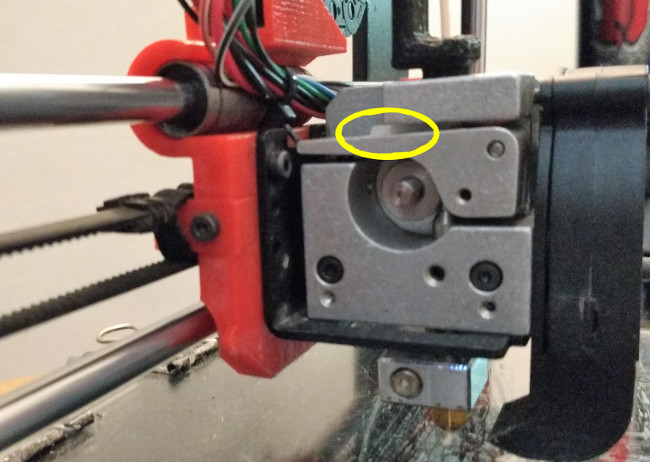
\includegraphics[width=0.5\textwidth,cfbox=azul_marcos 4pt 0pt]{FOTOS/SOLUCION1}
\caption*{HeatCore Extruder de BQ Hephestos y BQ Witbox}
\end{figure}
			\paragraph{Adicionando tensão entre a bobina e o extrusor}\mbox{}\\\\
Verificou-se que em alguns modelos de impressora é conveniente que, ao utilizar filamento flexível, exista alguma tensão entre a bobina e o extrusor, de modo a que o filamento não fique a colar.
\\\\
Para o conseguir pode fazer abrandar a bobina, de maneira que o extrusor tenha que afastar-se ligeiramente do filamento para desenrolá-lo. Também pode colocar um acessório semelhante ao da fotografia para alcançar o mesmo objetivo.
\begin{figure}[H]
\centering
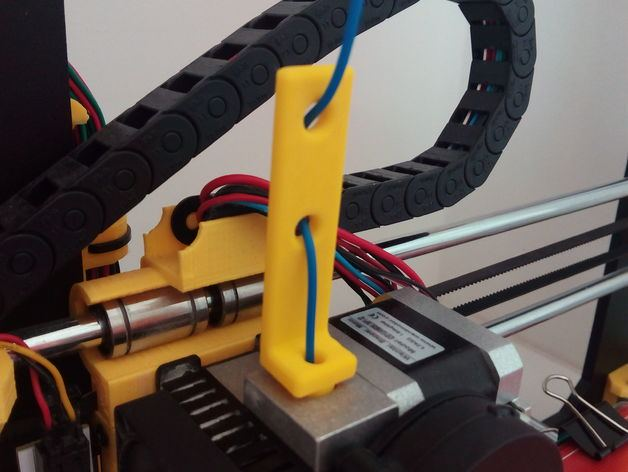
\includegraphics[width=0.5\textwidth,cfbox=azul_marcos 4pt 0pt]{FOTOS/SOLUCION2}
\caption*{Concebido para Extrusor BQ Unibody da BQ Hephestos}
\end{figure}
		\subsubsection{Substituir o seu extrusor por um otimizado}
Hoje em dia os filamentos flexíveis ficaram populares até ao ponto de não ser difícil que uma impressora de última geração não esteja preparada para os imprimir.
\\\\
Além disso, são muitos os desenhadores que criaram extrusores imprimíveis capazes de imprimir FlexiSMART e outros filamentos. Estes extrusores podem descarregar-se em páginas como a Thingiverse para serem impressos e montados em casa.
\\\\
Também são cada vez mais os extrusores comerciais preparados para imprimir filamentos flexíveis que se podem adquirir e montar nas nossas impressoras.
			\paragraph{Extrusores imprimíveis DIY}\mbox{}\\\\
Alguns destes extrusores são desenhados desde o zero e outros são modificações realizadas a partir de desenhos já existentes. Aqui apresentamos uma lista não exaustiva de desenhos de extrusores que podem ser descarregados da internet. Seguindo cada link poderá encontrar a lista de componentes completa, bem como as instruções de montagem e comentários de outros utilizadores.
\\\\
O hot-end que instalar no seu extrusor deve ter uma peça de teflon (PTFE) no seu interior, para evitar fricções e para que o FlexiSMART se imprima corretamente. O FlexiSMART foi testado com êxito nos seguintes hot-ends \footnote{Deve ter em conta que esses testes foram realizados com hot-ends originais e não podemos garantir o mesmo resultado nas réplicas destes.}:
\begin{itemize}
\item J-Head MKV-B
\item Budassnozzle V1.3
\item E3D v6
\item Leonnozzle V2
\end{itemize}
Dependendo da impressora que utilizar, alguns destes extrusores serão mais fáceis de instalar, dado que poderão substituir diretamente o extrusor original da máquina.
\begin{figure}[H]
    \centering
    \begin{subfigure}[b]{0.4\textwidth}
        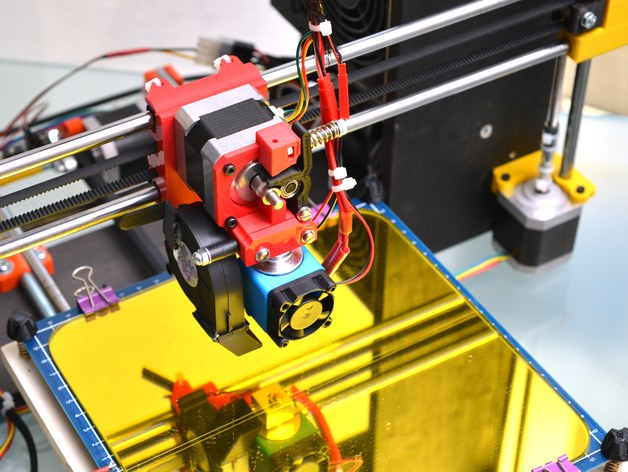
\includegraphics[width=\textwidth,cfbox=azul_marcos 4pt 0pt]{FOTOS/EXTRUSOR1}
		\caption*{\href{http://www.thingiverse.com/thing:147705}{{\footnotesize Direct-drive hinged extruder for E3D/J-Head hot-end (Prusa i3) by ffleury}}}
    \end{subfigure}
    ~ \qquad%add desired spacing between images, e. g. ~, \quad, \qquad, \hfill etc. 
      %(or a blank line to force the subfigure onto a new line)
    \begin{subfigure}[b]{0.4\textwidth}
        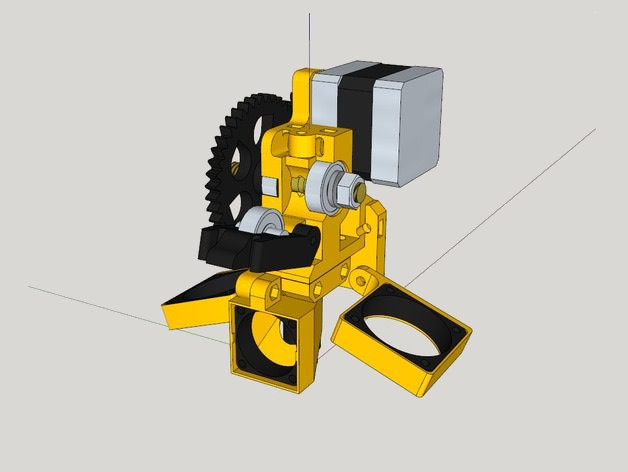
\includegraphics[width=\textwidth,cfbox=azul_marcos 4pt 0pt]{FOTOS/EXTRUSOR2}
		\caption*{\href{http://www.thingiverse.com/thing:512338}{{\footnotesize Wade L3K Extruder (prusa I3) compatible filament flexible By Skarab}}}
    \end{subfigure}
\end{figure}
\begin{figure}[H]
    \centering
    ~ %add desired spacing between images, e. g. ~, \quad, \qquad, \hfill etc. 
    %(or a blank line to force the subfigure onto a new line)
    \begin{subfigure}[b]{0.4\textwidth}
        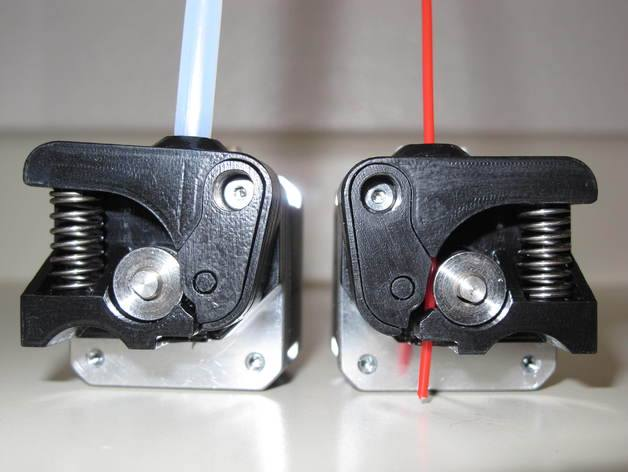
\includegraphics[width=\textwidth,cfbox=azul_marcos 4pt 0pt]{FOTOS/EXTRUSOR3}
		\caption*{\href{http://www.thingiverse.com/thing:403438}{{\footnotesize Printrbot Flexible Filament Direct Drive Extruder by thirdhorizon}}}
    \end{subfigure}
    ~ \qquad %add desired spacing between images, e. g. ~, \quad, \qquad, \hfill etc. 
    %(or a blank line to force the subfigure onto a new line)
    \begin{subfigure}[b]{0.4\textwidth}
        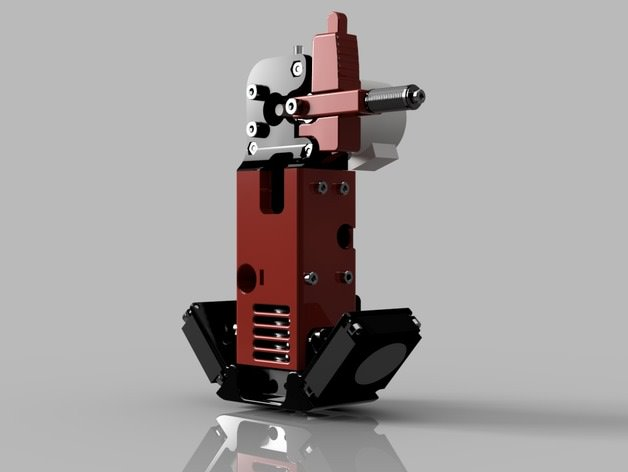
\includegraphics[width=\textwidth,cfbox=azul_marcos 4pt 0pt]{FOTOS/EXTRUSOR4}
		\caption*{\href{http://www.thingiverse.com/thing:1102900}{{\footnotesize Ultimaker 2 PG35L Direct Drive Extruder for 1.75mm E3D v6 Hotend by jasonatepaint}}}
    \end{subfigure}
\end{figure}
			\paragraph{Extrusores comerciais}\mbox{}\\\\
Adquirir um extrusor comercial é mais caro do que construir um caseiro, contudo, costumam ter melhor rendimento do que estes e são a melhor opção quando se utiliza filamento flexível de forma intensiva.
\\\\
Estes extrusores foram especificamente desenhados para evitar todos os problemas mencionados anteriormente e alguns podem extrudir FlexiSMART a velocidades superiores a 70 mm/s.
\begin{figure}[H]
    \centering
    \begin{subfigure}[b]{0.4\textwidth}
        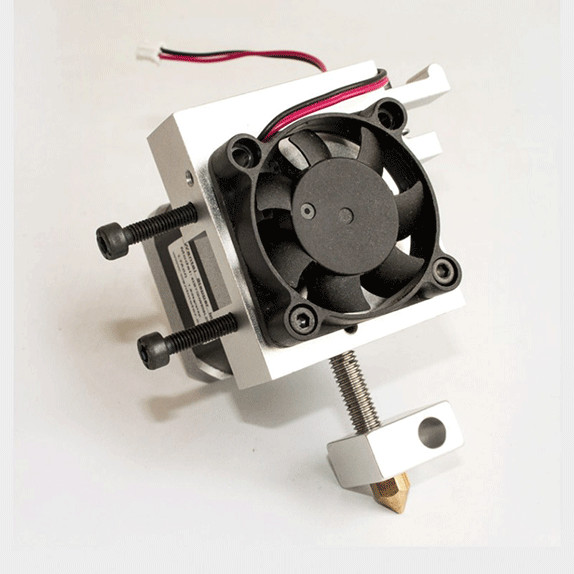
\includegraphics[width=\textwidth,cfbox=azul_marcos 4pt 0pt]{FOTOS/EXTRUSOR5}
		\caption*{\href{http://www.recreus.com}{{\footnotesize Recreus Extruder - Precio aprox. 100\euro}}}
    \end{subfigure}
    ~ \qquad%add desired spacing between images, e. g. ~, \quad, \qquad, \hfill etc. 
      %(or a blank line to force the subfigure onto a new line)
    \begin{subfigure}[b]{0.4\textwidth}
        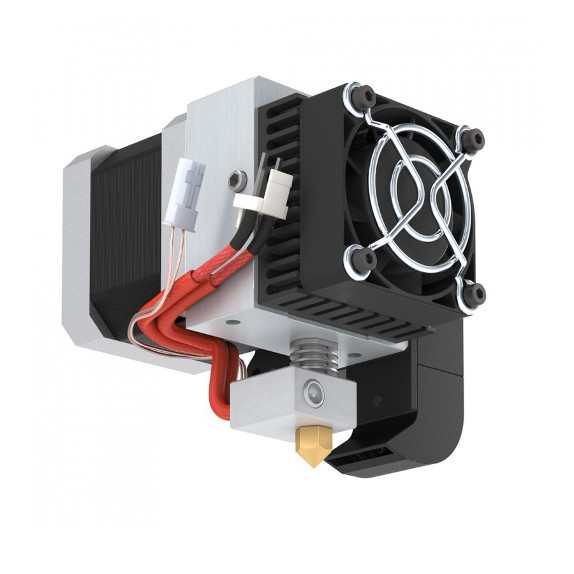
\includegraphics[width=\textwidth,cfbox=azul_marcos 4pt 0pt]{FOTOS/EXTRUSOR6}
		\caption*{\href{http://www.bq.es}{{\footnotesize BQ HeatCore DDG Extruder - Precio 140\euro}}}
    \end{subfigure}
\end{figure}
\begin{figure}[H]
    \centering
    ~ %add desired spacing between images, e. g. ~, \quad, \qquad, \hfill etc. 
    %(or a blank line to force the subfigure onto a new line)
    \begin{subfigure}[b]{0.4\textwidth}
        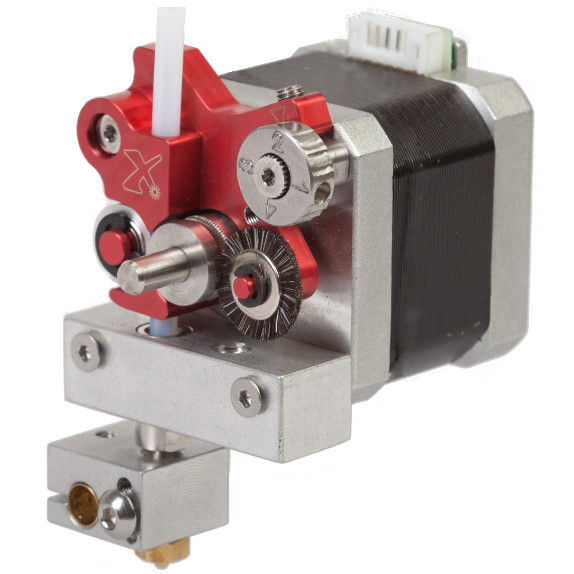
\includegraphics[width=\textwidth,cfbox=azul_marcos 4pt 0pt]{FOTOS/EXTRUSOR7}
		\caption*{\href{https://flexionextruder.com/}{{\footnotesize Flexion Extruder - Precio aprox. 140\euro}}}
    \end{subfigure}
    ~ \qquad %add desired spacing between images, e. g. ~, \quad, \qquad, \hfill etc. 
    %(or a blank line to force the subfigure onto a new line)
    \begin{subfigure}[b]{0.4\textwidth}
        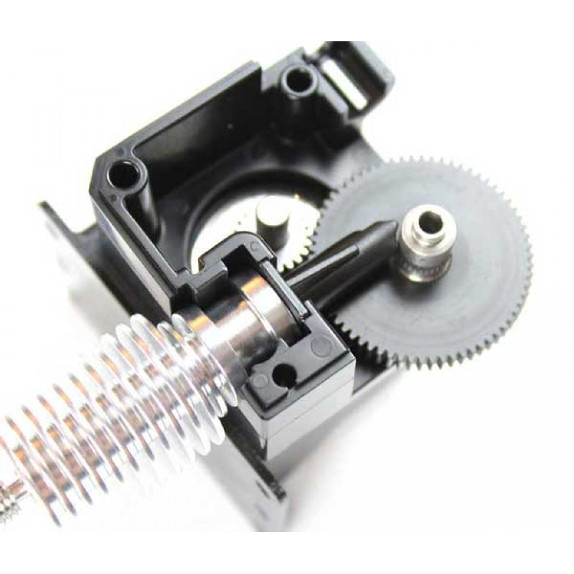
\includegraphics[width=\textwidth,cfbox=azul_marcos 4pt 0pt]{FOTOS/EXTRUSOR8}
		\caption*{\href{www.e3d-online.com}{{\footnotesize Titan Extruder - Precio aprox. 70\euro}}}
    \end{subfigure}
\end{figure}
\section{Conselhos para uma utilização ótima do FlexiSMART}
	\subsection{A retração}
A retração é uma técnica usada nas impressoras 3D FFF/FDM para melhorar o acabamento das peças. Consiste em ordenar ao extrusor que retire uns centímetros de filamento quando este mudar de posição, para evitar o stringing ou o surgimento de pequenos fios de filamento entre diferentes partes da peça que se está a imprimir.
\begin{figure}[H]
\centering
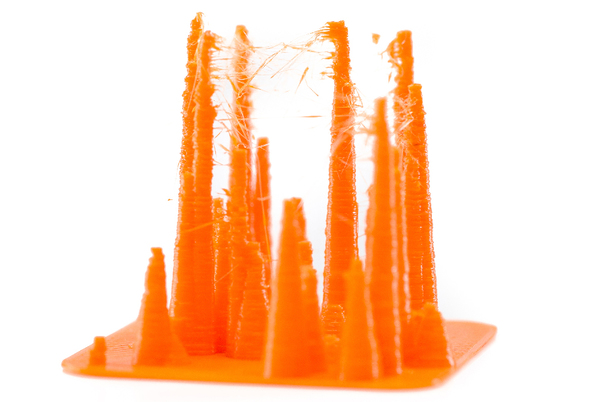
\includegraphics[width=0.5\textwidth,cfbox=azul_marcos 4pt 0pt]{FOTOS/RETRACCION1}
\caption*{Peça com problema de stringing}
\end{figure}
Quando se utilizam filamentos flexíveis pode acontecer que, ao procurar uma retração muito brusca, o filamento estique em vez de retroceder. Por isso é muito recomendável utilizar parâmetros de retração diferentes dos utilizados com filamentos rígidos.
\\\\
Os 2 parâmetros que podemos controlar na retração são o tamanho, ou quantidade linear em milímetros de filamento retraído, e a velocidade em mm/s da operação. Ambos os valores devem ser inferiores aos usados habitualmente. A forma ótima de calibrar estes valores é realizar testes para averiguar quais são os valores máximos que a sua impressora suporta ao imprimir com FlexiSMART. De qualquer modo, como ponto de partida, pode usar os valores por nós recomendados:
\begin{description}
\item [Tamanho da retração:] 1.5 mm
\item  [Velocidade da retração:] 40 mm/s
\end{description}
Dependendo da impressora, pode ser necessário desativar totalmente a retração.
	\subsection{Impressão sequencial}
Ao tratar-se de um filamento flexível, o FlexiSMART tem uma viscosidade diferente da de outros materiais quando alcança a sua temperatura de fusão. Por isso é mais propenso a deixar pequenos fios de filamento entre diferentes partes da peça quando o nozzle tem que se deslocar de um ponto para outro sem extrudir.
\begin{figure}[H]
\centering
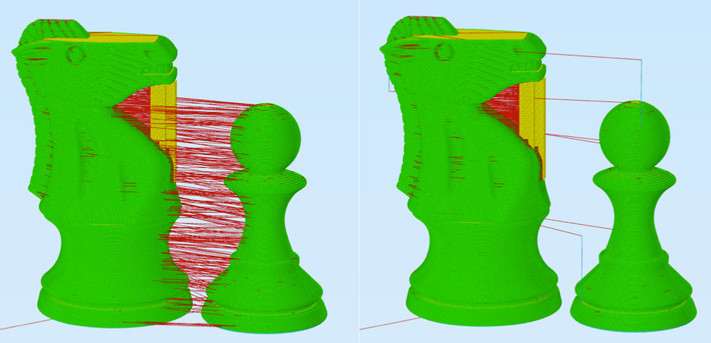
\includegraphics[width=0.5\textwidth,cfbox=azul_marcos 4pt 0pt]{FOTOS/SEQUENTIALPRINTING}
\caption*{Comparação das rotas de impressão entre impressão simultânea e sequencial}
\end{figure}
Além disso, quando se vão imprimir várias peças diferentes ao mesmo tempo, estes pequenos fios podem criar-se entre as peças, pois que o nozzle tem que saltar de umas para outras constantemente.
\\\\
Como já mencionámos anteriormente, este efeito pode reduzir-se fazendo uso da retração, mas é bastante recomendável que, além disso, se imprimam as diferentes peças de forma sequencial, em vez de simultaneamente.
\\\\
Com impressão sequencial referimo-nos a imprimir completamente uma peça antes de começar a imprimir a seguinte.
\\\\
Isto pode conseguir-se de 2 maneiras diferentes:
\begin{itemize}
\item A opção óbvia é imprimir só uma peça e, uma vez terminada, repetir a mesma impressão tantas vezes quantas se queira.
\item A segunda alternativa, mais avançada e com algumas limitações, é utilizar a opção oferecida por alguns programas de laminado, de imprimir uma peça de cada vez. O tamanho máximo das peças que podem ser impressas usando este método vem dado pelas dimensões do nozzle e pela disposição dos eixos da impressora. Recomendamos encarecidamente que se informe acerca de como usar estas opções, para não correr o risco de danificar a sua impressora. Pode fazê-lo através dos seguintes links:
\end{itemize}
\url{https://www.simplify3d.com/support/tutorials/multi-part-printing/}\\
\url{http://manual.slic3r.org/advanced/sequential-printing}\\
\url{https://ultimaker.com/en/community/3843-force-cura-to-print-objects-separately}
	\subsection{A primeira capa}
A primeira capa é o fundamento das restantes capas e pode marcar a diferença entre uma impressão satisfatória e uma impressão falhada.
\\\\
Ao imprimir com FlexiSMART há que dar uma atenção especial à primeira capa, já que, por vezes, uma impressora nivelada corretamente para imprimir com PLA ou ABS pode não o estar para imprimir FlexiSMART de forma adequada.
\\\\
Para saber se a impressora está corretamente nivelada há que observar atentamente como é que a máquina realiza a primeira capa.
\\\\
Se a primeira capa parece translúcida significa que o nozzle está demasiado próximo da plataforma e será necessário afastá-lo uns mícrons.
\\\\
Por outro lado, se a primeira capa parece despegar-se ou as pistas de material depositado apresentam espaços sem plástico entre elas será necessário aproximar o nozzle uns mícrons da plataforma.
\begin{figure}[H]
    \centering
    \begin{subfigure}[b]{0.3\textwidth}
        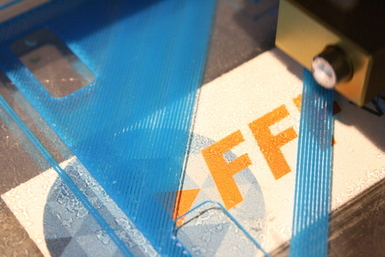
\includegraphics[width=\textwidth,cfbox=azul_marcos 3pt 0pt]{FOTOS/HOTENDALTO}
	\caption*{Nozzle demasiado lejos}
    \end{subfigure}
    ~ %add desired spacing between images, e. g. ~, \quad, \qquad, \hfill etc. 
      %(or a blank line to force the subfigure onto a new line)
    \begin{subfigure}[b]{0.3\textwidth}
        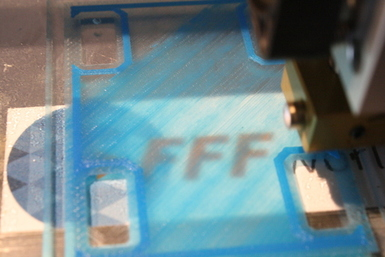
\includegraphics[width=\textwidth,cfbox=azul_marcos 3pt 0pt]{FOTOS/HOTENDBAJO}
	\caption*{Nozzle demasiado próximo}
    \end{subfigure}
    ~ %add desired spacing between images, e. g. ~, \quad, \qquad, \hfill etc. 
    %(or a blank line to force the subfigure onto a new line)
    \begin{subfigure}[b]{0.3\textwidth}
        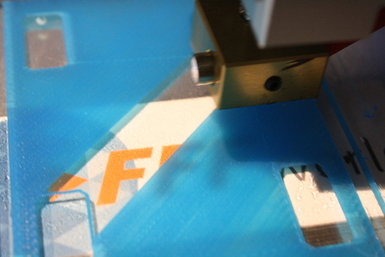
\includegraphics[width=\textwidth,cfbox=azul_marcos 3pt 0pt]{FOTOS/HOTENDPERFECTO}
	\caption*{Nozzle corretamente alinhado}
    \end{subfigure}
\end{figure}
Este ajuste pode realizar-se através de software, ajustando o z-offset no programa de laminado, ou regulando o mecanismo de nivelação da plataforma de impressão.
	\subsection{Conselhos de laminação}
		\subsubsection{A altura de capa}
A altura de capa determina a qualidade da peça e o tempo de impressão.
\\\\
Utilizando um nozzle de 0.4 mm temos verificado que a altura de capa ótima é de 0.2 mm. Com esta altura de capa conseguirá capas fortemente unidas com um acabamento superficial excelente.
		\subsubsection{Os top layers e perímetros}
Os top layers e os perímetros são o revestimento lateral e superior da peça. O número adequado para estes dependerá do infill e do uso que vai ser dado à peça.
\\\\
Com um infill alto, pode-se reduzir o número de top-layers para 3, dado que o enchimento da peça irá dar-lhes uma boa base de apoio. Utilizando valores de infill médios ou baixos é recomendável aumentar o número de top-layers para 5, para nos certificarmos de que a parte superior da peça fica completamente selada.
\\\\
Se a peça vai sofrer deformações é recomendável aumentar o número de shells ou perímetros horizontais. Aumentando o número de perímetros horizontais evitar-se-á que as paredes da peça possam desmanchar-se ao exercer pressão ou tração sobre elas.
\\\\
Estas recomendações são válidas quando se usa um nozzle de 0.4 mm e uma altura de capa de 0.2 mm. Se o tamanho do nozzle ou a altura da capa varia, o número de perímetros e top-layers ótimos também mudará.
\\\\
Convidamo-lo a realizar os seus próprios testes e partilhar o resultado connosco.
		\subsubsection{Influência do infill na flexibilidade}
A quantidade e o desenho do infill tem uma grande influência no grau de flexibilidade das peças impressas com FlexiSMART.
\\\\
Uma peça com um infill próximo de 100\% comportar-se-á como um bloco de borracha e pode ser uma boa opção para peças como silent-blocks ou spacers.
\\\\
Utilizando um infill de 15\% obterá peças brandas que poderão ser esmagadas e deformadas.
\\\\
O padrão do infill também afeta a flexibilidade e não se comporta da mesma forma que um infill retilíneo de um honeycomb (painel de abelha).  Convidamo-lo a realizar os seus próprios testes e escolher aquele que melhor se adequar ao seu projeto.
	\subsection{Utilização de um nozzle de maior tamanho}
A maior parte das impressoras utilizam de série um nozzle de 0.4 mm, um tamanho de nozzle que proporciona uma boa proporção velocidade/resolução. O FlexiSMART imprime-se perfeitamente com este tipo de nozzle, ainda assim é conveniente fazer uns retoques.
\\\\
O tamanho do nozzle limita a quantidade de material que pode ser extrudido por unidade de tempo. Ao utilizar filamentos rígidos este limite é maior, dado que se pode aumentar a velocidade e o próprio filamento suporta a pressão extra necessária para que o material saia pelo nozzle. Com o FlexiSMART, no entanto, o filamento comprime-se se esta pressão for demasiado alta e, em geral, deve ser impresso a velocidades menores.
\\\\
Por isso, se quer extrudir FlexiSMART a velocidades elevadas, é recomendável a utilização de um nozzle de maior tamanho, a partir de 0.6 mm. Utilizando um destes nozzles poderá imprimir muito mais rápido, com alturas de capa superiores, sacrificando um pouco a resolução.
\section{Quer apoiar o nosso projeto?}
Todos os membros FFF World adoram a impressão 3D e a comunidade maker. Sentimo-nos uns sortudos por poder trabalhar em projetos onde podemos pôr em prática a nossa paixão sincera. No futuro, gostaríamos de poder desenvolver mais materiais, mais cores, mais formatos. Definitivamente, gostaríamos de poder fazer crescer a nossa empresa.
\\\\
Para isso, uma das principais ações para nos ajudar, se quiser fazê-lo e estiver satisfeito com o filamento, é votar em nós no Amazon com 5 estrelas.
\begin{figure}[H]
\centering

\includegraphics[width=0.5\textwidth,cfbox=azul_marcos 1pt 0pt]{FOTOS/AMAZON_FIVE_STARS}
\caption*{¡Muchas gracias!}
\end{figure}
\subsection{Outros filamentos com excelentes propriedades agora disponíveis no Amazon}
\begin{description}
\item[FlexiSMART Tech:] Concebido para resistir à abrasão e ao desgaste de impressões técnicas.
\item[ABS Tech:] Efeito warping minimizado. Alto rendimento em aplicações técnicas.
\item[PETG Tech:] Máxima resistência mecânica. Resistente ao contacto com a água e os raios UV. Apto para uso alimentar.
\item[FilaMETAL:] PLA com carga metálica não abrasiva que dá um acabamento metálico espetacular às suas impressões.
\item[PC Tech:] Policarbonato com grande resistência à temperatura e com excelentes propriedades mecânicas.
\item[Nylon Tech:] Imprimível a baixa temperatura. Resistência aos choques com um certo grau de flexibilidade.
\item[PVA Tech:] Filamento solúvel em água indicado para ser utilizado como material de suporte. Excelente compatibilidade com PLA.
\item[HIPS Tech:] Filamento solúvel em limoneno, indicado para ser utilizado como material de suporte. Boa resistência mecânica e excelente compatibilidade com ABS.
\end{description}
%\section{Bibliografía}
%Esta guía no habría sido posible sin el conocimiento libre generado por la comunidad RepRap. Para la elaboración de esta guía se han %utilizado imágenes y contenido extraidos de los siguientes sitios web.
%\\\\
%\url{http://www.gyrobot.co.uk/blog/how-to-3d-print-with-flexible-filaments}\\
%\url{http://www.thingiverse.com/thing:1496895}\\
%\url{http://www.thingiverse.com/thing:247024}\\
%\url{http://www.thingiverse.com/thing:16319}\\
%\url{http://www.thingiverse.com/thing:779011}\\
%\url{http://www.thingiverse.com/thing:1102900}\\
%\url{http://www.thingiverse.com/thing:147705}\\
%\url{http://www.thingiverse.com/thing:222667}\\
%\url{http://www.thingiverse.com/thing:512338}\\
%\url{https://all3dp.com/common-3d-printing-problems-and-their-solutions/}\\
%\url{https://www.simplify3d.com/support/}\\
%\url{http://www.thingiverse.com/thing:508896}\\
%\url{http://www.thingiverse.com/thing:1187344}

\includepdf{PDF/PT_CONTRAPORTADA.pdf}
\end{document}
